\chapter{User Documentation} % User guide
\label{ch:user}

There are three main ways of using Histopathologic Cancer Detection program:
\begin{enumerate}
	\itemsep 0em
	\item Predicting tissue and cancer subtype of breast and colorectal tissue, i.e. predicting whether patient has breast or colorectal cancer or not
	\item Visualizing what Convolutional Neural Network learns, i.e. visualizing how network transforms input image, and which parts of input image lead to predicting tissue and cancer subtype
	\item Adding new datasets and networks in order to increase the scope of the program, and predict even more tissue and cancer subtypes
\end{enumerate}
In order to use the program to predict tissue and cancer subtype, or to visualize what CNNs learn, certain general software requirements are needed, while in order to expand the scope of the program, certain additional software requirements are needed.

\section{General Software Requirements}

Before running the program, Python3 programming language is required, along with following dependencies: 
\begin{itemize}
	\itemsep 0em
	\item h5py - interface to the HDF5 binary data format, which can store huge amounts of numerical data, and easily manipulate that data from NumPy (used to save and load network weights)
	\item Keras, Keras-Applications, Keras-Preprocessing, tensorflow - neural networks APIs, which can build and deploy machine learning applications (used to build and train neural networks)
	\item matplotlib, seaborn - data visualization libraries (used for visualization of datasets, neural networks and tissue and cancer subtype predictions)
	\item NumPy - library which provides support for large, multi-dimensional arrays
	\item opencv-python, Pillow, scikit-image - image processing libraries (used to load, process and save images)
	\item pandas - data analysis and manipulation library (used for loading datasets)
	\item PyQt5 - python binding of cross-platform GUI toolkit Qt, which contains substantial set of GUI widgets (used for implementing GUI part of the program)
	\item scikit-learn - machine learning library for predictive data analysis (used for its metrics in order to assess network performance)
\end{itemize}
If general software requirements are satisfied, program can be used to predict tissue and cancer subtypes, as well as to visualize network representations.

\section{Additional Software Requirements}

In order to replicate results of already existing networks, or to expand scope of the program by adding new datasets and training new networks, NVIDIA graphics card is required, along with the following:
\begin{itemize}
	\itemsep 0em
	\item NVIDIA CUDA toolkit - provides a development environment for creating high performance GPU-accelerated applications
	\item NVIDIA CUDA Deep Neural Network Library (cuDNN) - GPU-accelerated library of primitives for deep neural networks, which provides highly tuned implementations for standard routines
	\item tensorflow-gpu - GPU-enabled version of tensorflow library
\end{itemize}
Training convolutional neural networks requires large amount of computations, and in order to decrease training time, networks are trained on GPU (it is not feasible on CPU, as GPU training is multiple times faster).

\section{Runnig the Program}

After running the program, new window appears (\textcolor{red}{\autoref{fig:startup}}).

\begin{figure}[h]
	\centering
	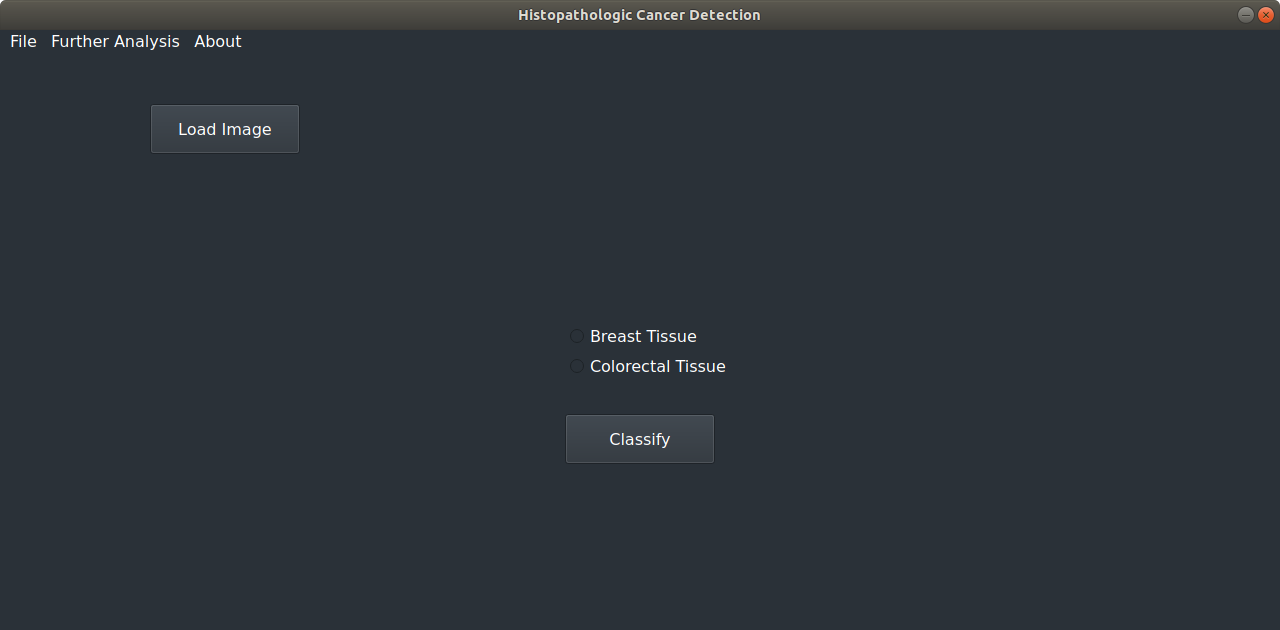
\includegraphics[scale=0.3]{startup_window.png}
	\caption{Main window of Histopathologic Cancer Detction program}
	\label{fig:startup}
\end{figure}

From here, it is possible to:
\begin{enumerate}
	\itemsep 0em
	\item Inspect datasets and networks
	\item Load histopathologic slide of breast or colorectal tissue and predict the tissue and cancer subtype
	\item Further visualize network representations by analyzing heatmaps of class activations, filters of convolutional layers and intermediate activations
\end{enumerate}

\section{Inspecting Datasets}

In order to find basic information about datasets, which include sample images from dataset, tissue and cancer subtypes, as well as number of images per category, go to \emph{About $\rightarrow$ About\;Datasets} and choose dataset (\textcolor{red}{\autoref{fig:inspectdataset}}). In current implementation there are two datasets available: BreakHis and NCT-CRC-HE-100K.
\clearpage

\begin{figure}[h]
	\centering
	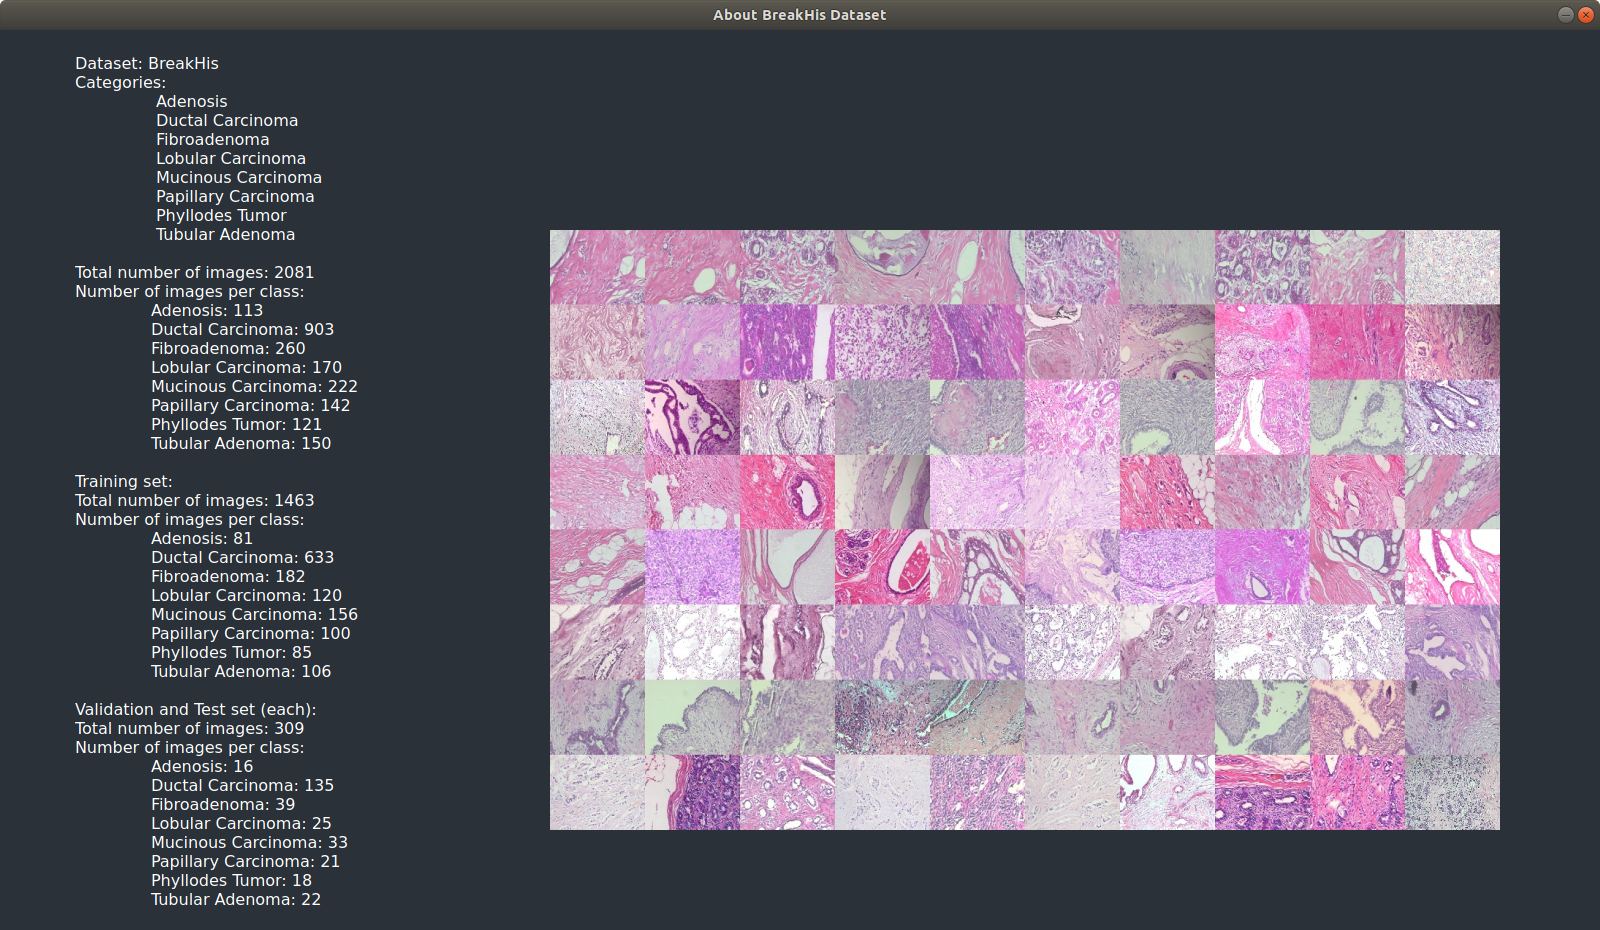
\includegraphics[scale=0.25]{inspect_dataset.png}
	\caption{BreakHis Dataset basic information}
	\label{fig:inspectdataset}
\end{figure}

\section{Inspecting Networks}

In order to find basic information about networks, which include network architecture and network performance on training, validation and test datasets (accuracy, loss and confusion matrix), go to \emph{About $\rightarrow$ About\;Models} and choose network (\textcolor{red}{\autoref{fig:inspectdataset}}). In current implementation there are two networks available: CNNSimple and VGG19Simple.

\begin{figure}[h]
	\centering
	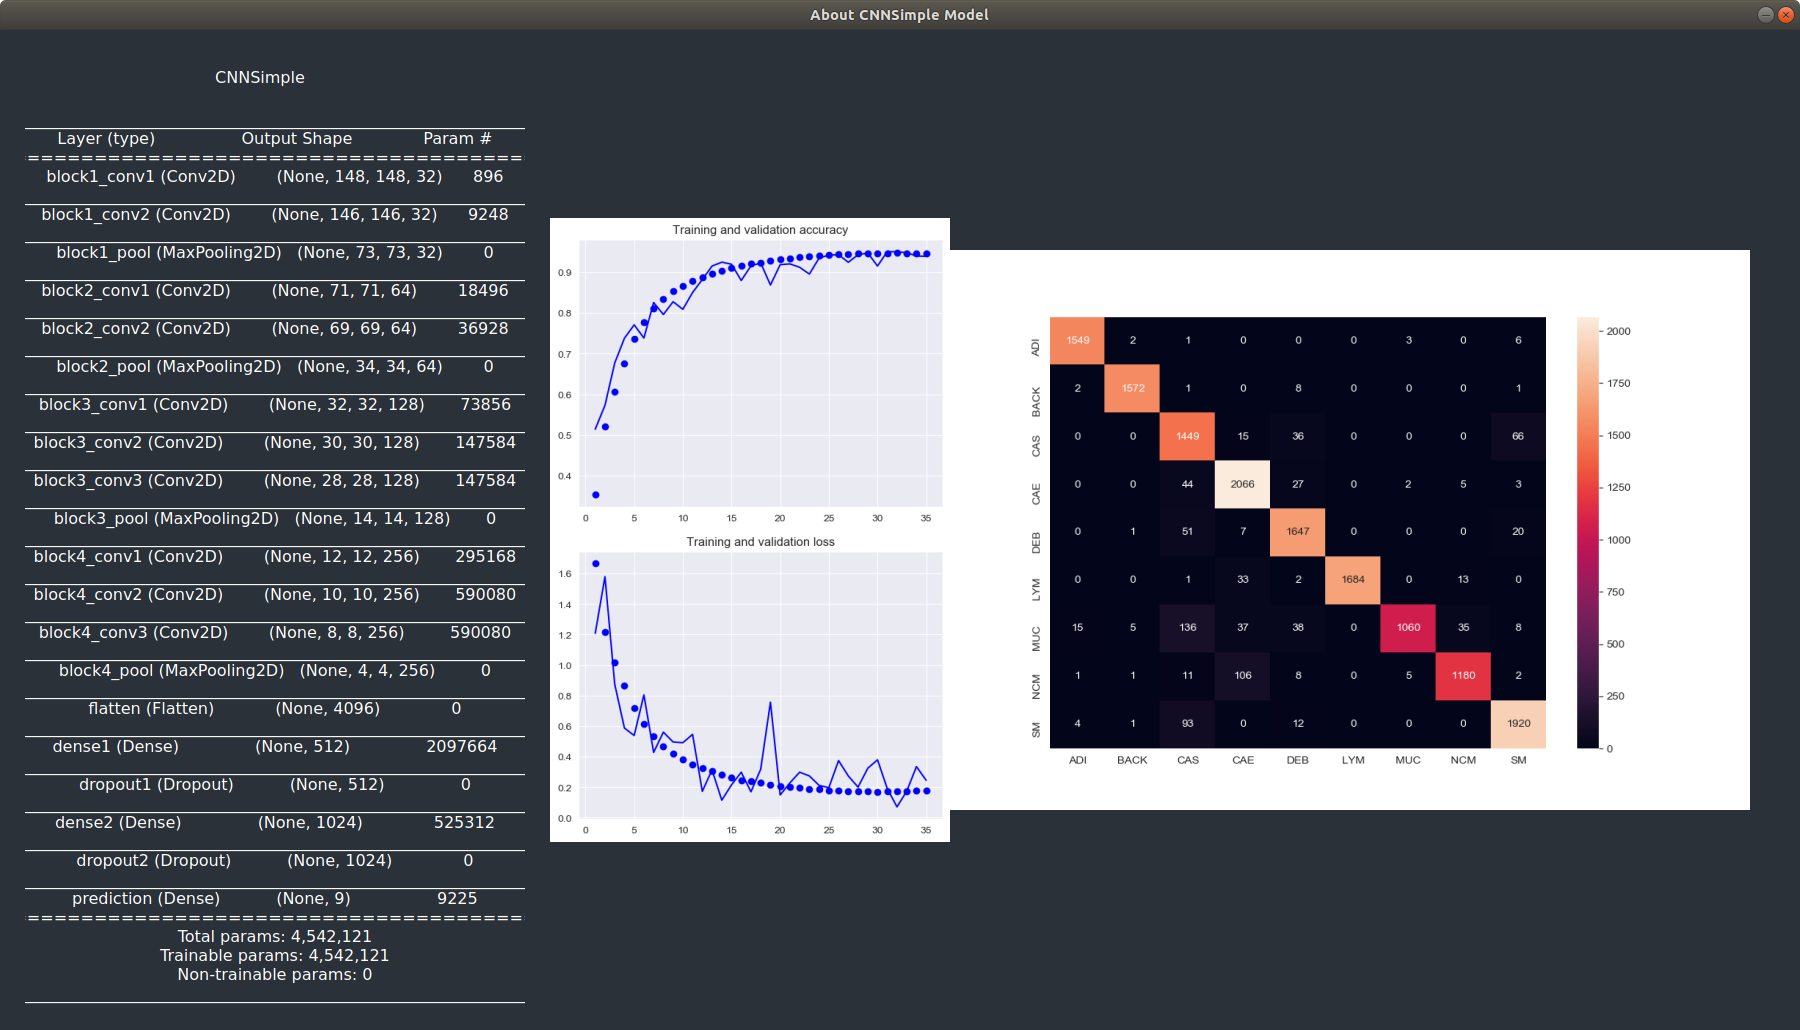
\includegraphics[scale=0.2]{inspect_network.png}
	\caption{CNNSimple Network basic information}
	\label{fig:inspectdataset}
\end{figure}

\section{Basic Use: Predicting Tissue Type}

Main use of the Histopathologic Cancer Detection program is to make it easy and fast to load histopathologic slide and get a prediction on tissue and cancer subtype. In order to load a histopathologic slide, click on \emph{Load\; Image}, and select histopathologic slide for which the prediction is required. Next, select a tissue type of the slide by clicking on \emph{Breast\;Tissue} or \emph{Colorectal\;Tissue}. Afterwards, in order to get tissue and cancer subtype, along with probabilities graph, press \emph{Classify} button (\textcolor{red}{\autoref{fig:predict}}).

\begin{figure}[h]
	\centering
	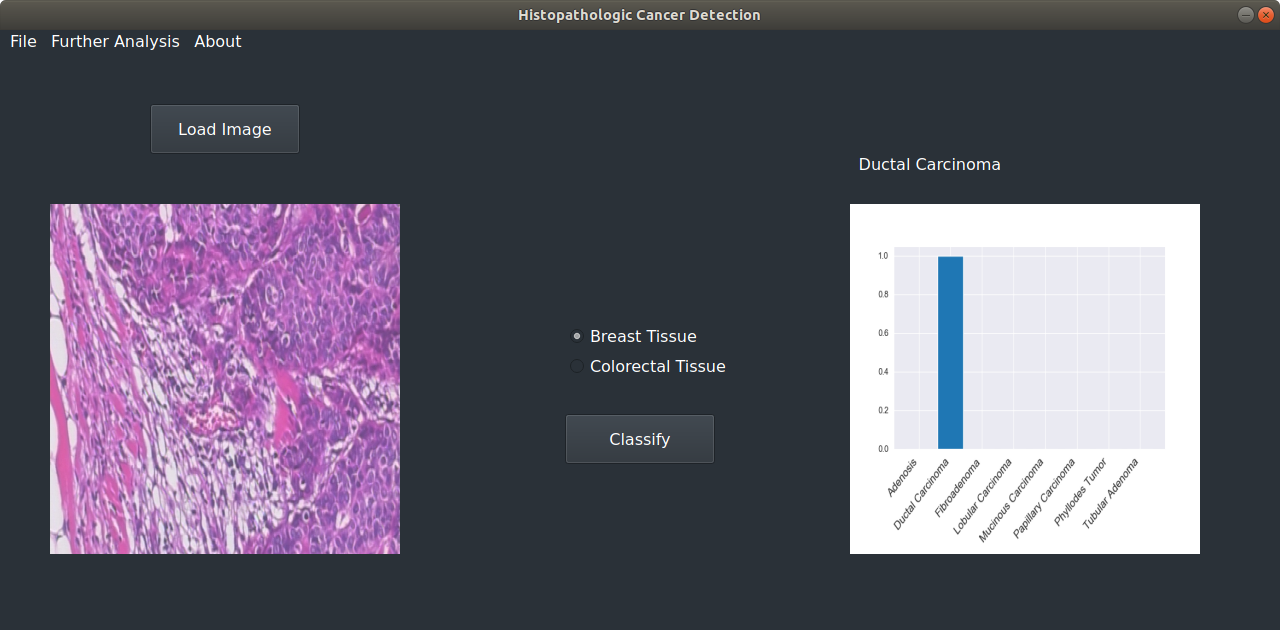
\includegraphics[scale=0.33]{predict.png}
	\caption{Prediction of input histopathologic slide of breast tissue to be ductal carcinoma}
	\label{fig:predict}
\end{figure}

\section{Advanced Use: Visualizing Network Representations}

Deep neural networks are highly complex models which have great expressive power and can achieve high accuracy while solving wide range of problems. Unfortunately, with high complexity comes low interpretability, which presents issue, especially in deep learning applications to healthcare. Fortunately, there are several methods to inspect convolutional neural networks, and interpret their output. In this paper, I covered three of them: visualizing heatmaps of class activations, visualizing filters of convolutional layers and visualizing intermediate activations.

\subsection{Visualizing Heatmaps of Class Activations}

Different parts of an image have different weights in networks decision on tissue and cancer subtype classification, and because of that, we can highlight which parts of an image have the highest influence on the networks output. This class of methods is called class activation map visualization, and it produces heatmaps of class activations over input images. A class activation heatmap is a 2D grid of scores associated with a specific output class, computed for every location in any input image, indicating how important each location is with respect to the class under consideration. In order to produce heatmap, go to \emph{Further Analysis $\rightarrow$ Heatmap} (\textcolor{red}{\autoref{fig:heatmap}}).

\begin{figure}[h]
	\centering
	\begin{minipage}{.5\textwidth}
		\centering
		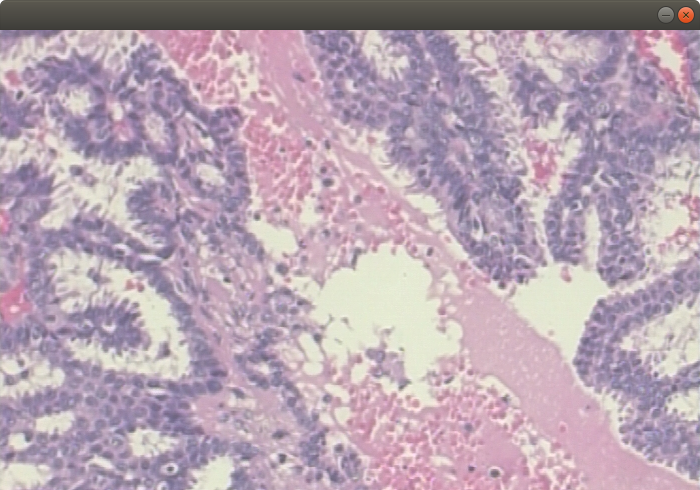
\includegraphics[scale=0.25]{input.png}
		\captionof{figure}{Input image of breast tissue}
		\label{fig:input}
	\end{minipage}%
	\begin{minipage}{.5\textwidth}
		\centering
		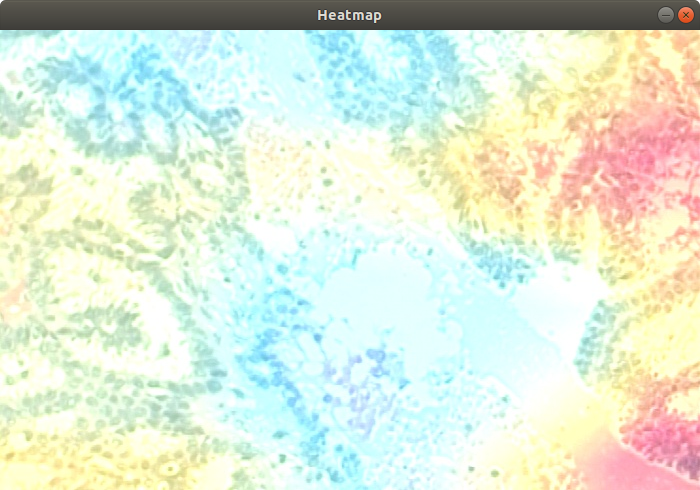
\includegraphics[scale=0.25]{heatmap.png}
		\captionof{figure}{Heatmap of class activations on input image}
		\label{fig:heatmap}
	\end{minipage}
\end{figure}

\subsection{Visualizing Intermediate Activations}

Visualizing intermediate activations consists of displaying the feature maps that are output by various convolution and pooling layers in a network, given a certain input (the output of a layer is often called its activation, the output of the activation function). This gives a view into how an input is decomposed into the different filters learned by the network. In order to visualize intermediate activations of layers, go to \emph{Further Analysis $\rightarrow$ Class Activations}. Next choose which network layer's intermediate activations should be visualized, along with channel number, or 'all', for visualizing all of layer's channels  (\textcolor{red}{\autoref{fig:interact}}).
\clearpage

\begin{figure}[h]
	\centering
	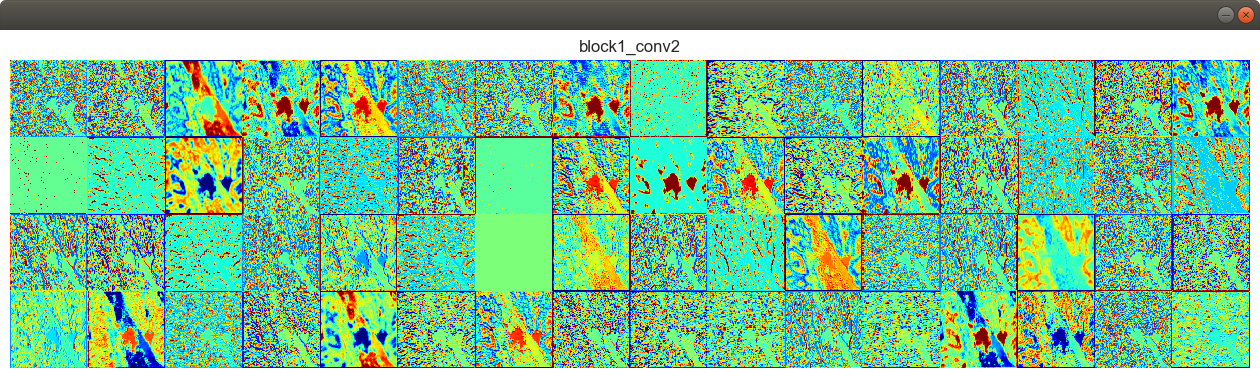
\includegraphics[scale=0.33]{layer_activations.png}
	\caption{Every channel of second convolutional layer of VGG19Simple on a breast tissue input (\textcolor{red}{\autoref{fig:input}}).}
	\label{fig:interact}
\end{figure}

\subsection{Visualizing Filters of Convolutional Layers}

Further analysis is not only dependent on an input image, as we can also inspect feature exractors (filters) of convolutional layers by displaying patterns on which each filter is supposed to respond to. This can be done with gradient ascent in input space : applying gradient descent to the value of the input image of a convnet so as to maximize the response of a specific filter, starting from a blank input image. The resulting input image will be one that the chosen filter is maximally responsive to. In order to visualize filters of convolutional layers, go to \emph{Further Analysis $\rightarrow$ Network Filters}.  Next choose which network convolutional layer's filters should be visualized, along with filter number, or 'all', for visualizing all of layer's filters  (\textcolor{red}{\autoref{fig:filters}}).

\begin{figure}[h]
	\centering
	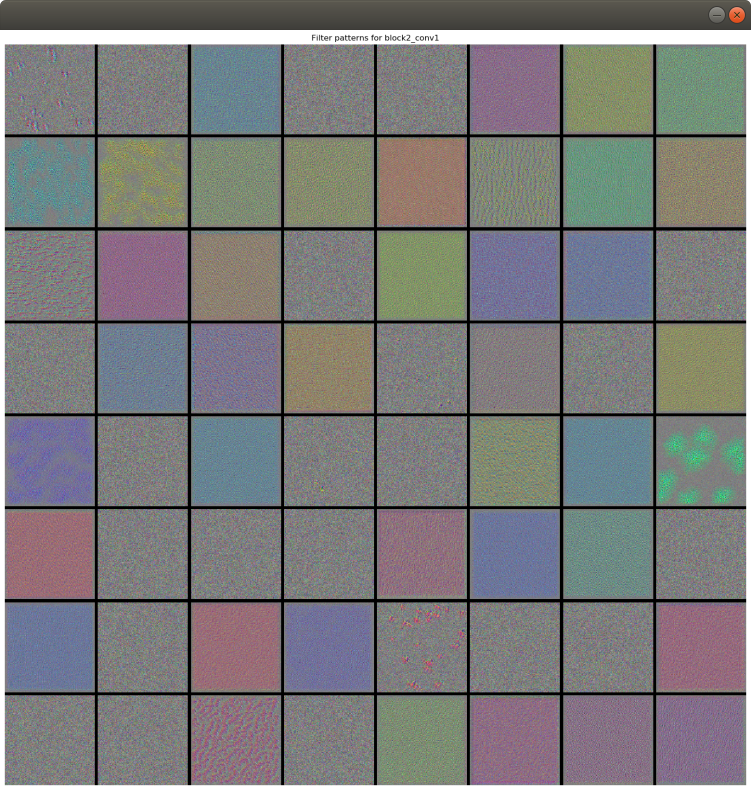
\includegraphics[scale=0.25]{filters.png}
	\caption{Filter patterns for second convolutional layer of CNNSimple network}
	\label{fig:filters}
\end{figure}

\clearpage

\section{Saving Results}
After all predictions have been made, and all further analysis has been conducted, in order to save the results, i.e. save all the images created during the program's execution, go to \emph{File $\rightarrow$ Save}.
